
%% bare_conf.tex
%% V1.4b
%% 2015/08/26
%% by Michael Shell
%% See:f
%% http://www.michaelshell.org/
%% for current contact information.
%%
%% This is a skeleton file demonstrating the use of IEEEtran.cls
%% (requires IEEEtran.cls version 1.8b or later) with an IEEE
%% conference paper.
%%
%% Support sites:
%% http://www.michaelshell.org/tex/ieeetran/
%% http://www.ctan.org/pkg/ieeetran
%% and
%% http://www.ieee.org/

%%*************************************************************************
%% Legal Notice:
%% This code is offered as-is without any warranty either expressed or
%% implied; without even the implied warranty of MERCHANTABILITY or
%% FITNESS FOR A PARTICULAR PURPOSE!
%% User assumes all risk.
%% In no event shall the IEEE or any contributor to this code be liable for
%% any damages or losses, including, but not limited to, incidental,
%% consequential, or any other damages, resulting from the use or misuse
%% of any information contained here.
%%
%% All comments are the opinions of their respective authors and are not
%% necessarily endorsed by the IEEE.
%%
%% This work is distributed under the LaTeX Project Public License (LPPL)
%% ( http://www.latex-project.org/ ) version 1.3, and may be freely used,
%% distributed and modified. A copy of the LPPL, version 1.3, is included
%% in the base LaTeX documentation of all distributions of LaTeX released
%% 2003/12/01 or later.
%% Retain all contribution notices and credits.
%% ** Modified files should be clearly indicated as such, including  **
%% ** renaming them and changing author support contact information. **
%%*************************************************************************


% *** Authors should verify (and, if needed, correct) their LaTeX system  ***
% *** with the testflow diagnostic prior to trusting their LaTeX platform ***
% *** with production work. The IEEE's font choices and paper sizes can   ***
% *** trigger bugs that do not appear when using other class files.       ***
%                       ***
% The testflow support page is at:
% http://www.michaelshell.org/tex/testflow/



\documentclass[conference]{IEEEtran}


% *** CITATION PACKAGES ***
%
\usepackage{cite} % cite.sty was written by Donald Arseneau
% The latest version can be obtained at:
% http://www.ctan.org/pkg/cite
% The documentation is contained in the cite.sty file itself.

\usepackage{xspace}
\usepackage{subfigure}
\usepackage{url}
\usepackage{hyperref}

% *** GRAPHICS RELATED PACKAGES ***
%
\ifCLASSINFOpdf \usepackage[pdftex]{graphicx} \usepackage{wrapfig} % declare the
\graphicspath{{pic/}} % and their extensions so you won't have to specify these
\DeclareGraphicsExtensions{.pdf,.png} \else % or other class option (dvipsone,
% dvipdf, if not using dvips). graphicx
% will default to the driver specified in the system graphics.cfg if no
% driver is specified.
% \usepackage[dvips]{graphicx}
% declare the path(s) where your graphic files are
% \graphicspath{{../eps/}}
% and their extensions so you won't have to specify these with
% every instance of \includegraphics
% \DeclareGraphicsExtensions{.eps}
\fi

% correct bad hyphenation here
% \hyphenation{op-tical net-works semi-conduc-tor}

\usepackage{textcomp} %\usepackage{svg}
%\setsvg{inkscape = inkscape -z -D, svgpath = svgs/}

\newcommand{\toolname}{Perquimans\xspace} \newcommand{\toolnameend}{Perquimans}
\newcommand{\toolnameposs}{Perquimans' }

\begin{document} \title{\toolnameend: A Tool for Visualizing Patterns of
		Spreadsheet Function Combinations}
	
	
	% author names and affiliations
	% use a multiple column layout for up to three different
	% affiliations
	\author{ \IEEEauthorblockN{Justin Middleton and Emerson Murphy-Hill}
		\IEEEauthorblockA{North Carolina State University, Raleigh, USA\\ jamiddl2@ncsu.edu, emerson@csc.ncsu.edu }}
	
	% use for special paper notices
	%\IEEEspecialpapernotice{(Invited Paper)}
	
	% make the title area
	\maketitle
	
	% As a general rule, do not put math, special symbols or citations
	% in the abstract
	\begin{abstract} Spreadsheet environments offer many
		functions to manipulate data, which users can combine into
		complex formulae. However, for both researchers and practitioners who want to
		study formulae to improve spreadsheet practices, anticipating these
		combinations is difficult. Therefore, we developed \toolnameend, a tool that
		analyzes spreadsheet collections to visualize patterns of function combination
		as an interactive tree, representing both the most common and most anomalous
		patterns of formula construction and their contexts. Using spreadsheets from
		the Enron corpus, we conduct a case study and a user study to explore
		\toolnameposs various applications, such as those in flexible smell
		detection and spreadsheet education.
		
	\end{abstract}
	
	\section{Introduction} Spreadsheets surround us. They are vital to
	industry and academia alike, supporting as much as 95\% of U.S. financial firms
	use them daily~\cite{panko2008sarbanes} and empowering teachers to track
	research and students' grades~\cite{ko2011state}. This flexibility boosts their
	allure: while a novice can work with basic offerings, advanced users can choose
	among the hundreds of specialized functions to fulfill a wide range of needs,
	from complex statistics to text manipulation~\cite{nardi1990spreadsheet}. As
	such, it should be no surprise that tens of millions of workers rely on these
	programs daily~\cite{scaffidi2005estimating}.
	
	However, this ubiquity is not without danger; as more people make larger and
	more complex spreadsheets, the cost of failure grows too. The European
	Spreadsheet Risks Interest Group (EuSpRIG) documents many horror stories of
	spreadsheets gone wrong\footnote{http://www.eusprig.org/horror-stories.htm},
	where consequences range from the profuse loss of money to the inaccurate
	outcomes of elections to the creation of extensive political initiatives based
	on flawed economics. Even if most spreadsheet errors are relatively benign,
	poor spreadsheet practice can risk millions, if not billions, of
	dollars~\cite{powell2009impact}.
	
	Fortunately, spreadsheet researchers address these dangers by amassing
	spreadsheet collections from diverse sources, industrial to academic, so
	they can study how people use spreadsheets. Collections like
	EUSES~\cite{fisher2005euses}, Fuse~\cite{barik2015fuse}, and the Enron
	corpus~\cite{hermans2015enron} have already produced valueable research, such
	as the documentation of code smells in spreadsheet
	environments~\cite{hermans2012detecting}~\cite{jansen2015code} or the creation
	of grammars to describe every possible spreadsheet program in
	Excel~\cite{aivaloglou2015grammar}. Additionally, some research compares these
	collections to discover variation in spreadsheet techniques over time and
	location~\cite{jansen2015enron}.
	
	The value of spreadsheets demands that we design tools to better understand
	these datasets and simplify complexities we find in them. One such complexity
	is formula construction; functions are an important part of using spreadsheets
	efficiently, yet the number of potential combinations is massive considering
	that Excel boasts over 400 functions. Tools that explore these combinations in
	practice can aid researchers in understanding how people program and in
	educating new generations of spreadsheets users on how to work best.
	
	This paper contributes such a tool, \toolnameend, that attempts to fulfill this
	need for better exploration of spreadsheet corpora. Working with spreadsheets
	in Excel, \toolname focuses primarily on the functions, like SUM and IF and
	hundreds more, which are the building blocks of formulae that determine values
	across a spreadsheet. The tool creates an interactive visualization which
	captures how people combine these functions, quantifying the broad patterns of
	function nesting while also capturing anomalous formulae and their locations.
	
	We also discuss several of the key decisions we faced during design, such as
	what to do with a sheet's redundant formulae or how to represent optional
	arguments, and we describe how our overall design goals both helped and
	hindered this process. We then apply the tool to a number of case studies to
	evaluate how much it could contribute to several different contexts, most
	notably code smell detection and spreadsheet education. To better understand
	how people might use \toolnameend, we also conducted a user study to judge how
	usable and intuitive the tool actually is. This grounds the discussion of its
	potential uses while also underscoring some of its inherent limitations and
	setting the way for future extensions and improvements upon the concept.
	
	\section{Related Work} \label{related-work} Visualizations excel for their
	ability to communicate information quickly and
	efficiently~\cite{baeza1999modern}; the visualization of spreadsheets,
	therefore, offers much room for research. Several previous tools work
	within a spreadsheet, clarifying connections between the visible
	values in cells, the formulae that produce them, and the dependencies between
	cells that inform them. Igarashi and colleague's fluid
	visualizations~\cite{igarashi1998fluid}, for example, do this by imposing
	lines, color, and animation over the spreadsheet to visually explain these
	tangled connections. Likewise, Clermont explored ways of grouping cells by
	color and border that were related through similar functions, neighbors, or
	references~\cite{clermont2003scalable}, and Hipfl extended this work by
	incorporating the layouts and labels of spreadsheets~\cite{hipfl2008using}.
	
	Other tools focus on creating visualizations external to the sheets. Hermans
	and colleagues address a spreadsheet programmer's information needs by making
	dataflow diagrams from individual sheets through the tools
	GyroSAT~\cite{hermans2011supporting} and Breviz~\cite{hermans2011breviz}.
	\toolname is among this type, creating standalone visualizations about
	spreadsheets instead of drawing connections inside the spreadsheet itself. In
	contrast to the other visualization work, our work focuses on representing
	functions and how they combine into complex formulae, rather than exploring the
	data structures of any particular spreadsheet. 
	
	Many other tools inspect the structure of formulae but from the
	perspective of finding bad design.  Following Fowler's initial description of
	code smells in object-oriented design~\cite{fowler2009refactoring}, many
	researchers have applied similar observations to spreadsheets and have
	cataloged classes of problematic
	formulae~\cite{hermans2012detecting}~\cite{cunha2012towards}~\cite{asavametha2012detecting}, often accompanying them with detection tools~\cite{abreu2014smelling} and investigations into real datasets~\cite{jansen2015code}. For example, Hermans, leveraging her work with the aforementioned dataflow diagrams, has worked with assessing common inter-worksheet smells, such as feature envy and inappropriate intimacy, wherein references between worksheets (rather than cells) in a file suggest a problem~\cite{hermans2012detectinginter}. Other tools, like Badame's Excel refactoring~\cite{badame2012refactoring}, are concerned more with understanding the formula in service of changing them. Though \toolname supports the search for bad design, as we will see, the tool itself takes a much more agnostic approach in presentation, offering examples without regard for design quality.

	Implicit in this study is an exploration of the Excel API and how people use
	it. Previous research, such as the first study on the Enron
	spreadsheets~\cite{hermans2015enron} or in its comparison with the EUSUS
	corpus~\cite{jansen2015enron}, quantifies how often users employ certain
	functions but not how they combine them. Researchers have applied such
	questions to other contexts as well, such as Murphy and colleague's study into
	how Java developers use Eclipse and what commands they use most
	often~\cite{murphy2006java}. Others focus on the documentation of the API
	itself: Robillard and DeLine, for example, conducted a series of surveys and
	interviews to diagnose common problems with learning APIs. They found that
	code examples, which is one of the focuses of this tool, is one of the most important
	aids to have in learning a new system~\cite{robillard2011field}. Though this
	paper applies the tool to the Enron corpus specifically, the tool itself is not
	limited to this; it can be readily applied to any collection of Excel
	spreadsheets a user gives it.
	
	\section{Approach}
	
	\subsection{Design Goals} \label{goals} In visualizing the spreadsheet data, we
	set out a few core goals for what the tool should accomplish. Furthermore, with
	these goals, we also considered the likely challenges of achieving those goals
	and particular outcomes which we considered beyond the scope of the research.
	We present both sides of these goals below:
	
	\begin{itemize}
		
		\item [1] \textbf{Unbiased Exploration} First, provide an interactive
		environment for free exploration. There are a lot of data in some of these
		spreadsheet corpora, and the user should be able to pick for themselves which
		to explore while ignoring the rest. Second, avoid judgments about good and bad
		design. Though users may certainly approach the tool with the intention of
		exploring particular formulae, a formula visualization tool will not
		prioritize any on metrics of good or bad practice.
		
		\item [2] \textbf{Uncluttered Quantification} \toolname should emphasize the
		quantitative patterns in formula construction and address the questions of how
		often the spreadsheet programmers used a certain function and where they used
		it. To do this, it must show metrics, such as frequency of use and depth of
		function nesting, but it must not overwhelm with numbers. Though everything
		should be accessible in accordance with the first goal, we should reduce noise with our design.
		
		\item [3] \textbf{Informative Qualification} The tool should promote a qualitative understanding of the patterns by providing concrete instances of relevant
		formulae from the corpus. Ideally, it should even direct users to the exact
		cell in the spreadsheets where the formula was used, contextualizing the
		functions.
		
	\end{itemize}
	
	\subsection{Walkthrough of the Tool} \label{sec:walkthrough}Before discussing
	\toolnameposs development, we will give a basic example of how to use
	it. We will work from the visualization built on the Enron
	corpus to answer this question: \textit{ What kinds of functions do people use
		to define the condition in an \texttt{IF} function?}
	
	In Excel, the \texttt{IF} functions is one of the logical functions: given a condition
	as the first argument that evaluates to either true or false, it takes on the
	value of either the second or third argument respectively. Or, as the
	documentation writes out, ``\texttt{IF(Something is True, then do something, otherwise
	do something
	else)}"\footnote{\href{https://support.office.com/en-us/article/IF-function-69aed7c9-4e8a-4755-a9bc-aa8bbff73be2}{https://support.office.com/en-us/article/IF-function-69aed7c9-4e8a-4755-a9bc-aa8bbff73be2}}. Furthermore, the third argument is optional; if left out, the function will return a default ``FALSE" value if necessary. Examples of this function in practice can be seen in Figure~\ref{fig:ifexample}.
	
	\begin{figure}[h] \centering 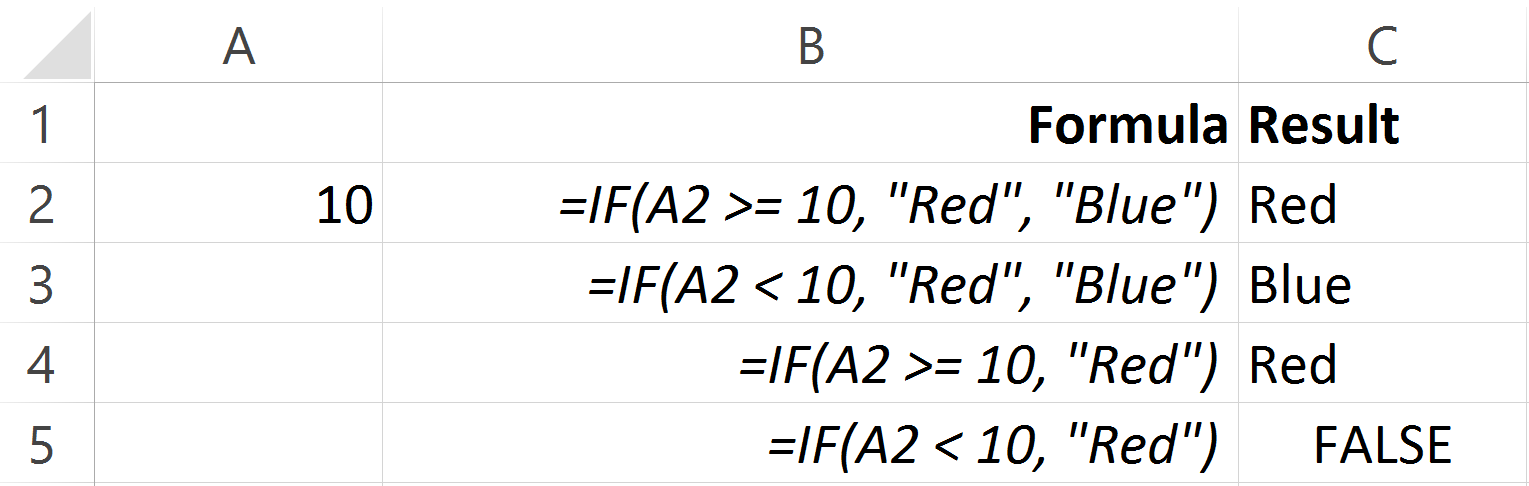
\includegraphics[width=\columnwidth]{ifExample}
		\caption{Configurations of the IF function} \label{fig:ifexample} \end{figure}
	
	When the user first approaches the tree for a given top-level function -- that
	is, a function nested within none other -- only a few nodes are visible, as
	shown in Figure~\ref{fig:startpic}. 
	
	\begin{figure}[h] \centering 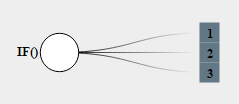
\includegraphics[width=.4\columnwidth]{start} \caption{How the
			IF tree looks at the start} \label{fig:startpic} \end{figure}
	
	The visualization so far comprises two types of nodes. The first are the
	circles 
\includegraphics{glossary-greenonly}, which represents a discrete
	function in the formula. These nodes are sized according to their frequency relative
	to the number of times the root function appeared. The second kind of node are
	the numbered squares 
\includegraphics{glossary-blue}, which represent the
	positions of arguments within its parent function. Looking back at the tree, we
	can confirm that \texttt{IF} functions in this dataset had at most three arguments
	passed into them, which corresponds with its specifications in the API. 
	
	Knowing that the first argument of \texttt{IF} contains the conditionals, we click on
	the square labeled ``1" to explore. When the tool finds more than 10 unique
	arguments in a position, it saves space by displaying only the first ten and
	includes an option to display the rest by clicking the arrow
	
\includegraphics{glossary-arrow}.
	
	\begin{figure}[h] \centering 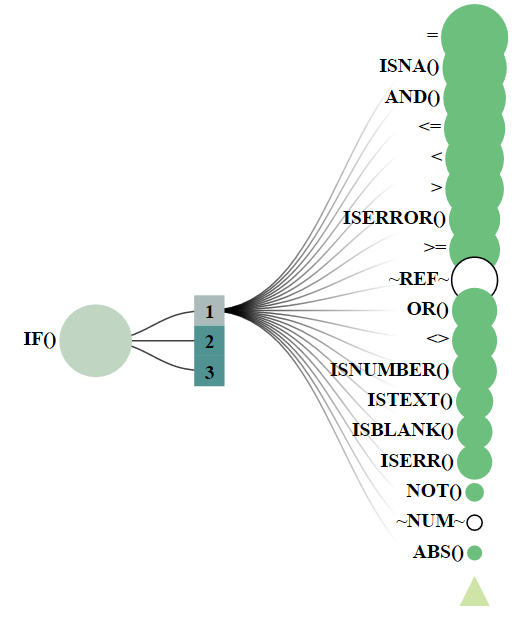
\includegraphics[width=0.7\columnwidth]{IFexpand}
		\caption{First argument of the \texttt{IF} tree} \label{fig:expandif} \end{figure}
	
	In Figure~\ref{fig:expandif}, we see that \texttt{IF}'s first arguments are most often comparison operators,
	such as = and $\le$, and boolean-returning functions, like \texttt{ISNA} and \texttt{AND}. Of these,
	simple equality is the most common and ABS is the least. From here, we
	can further explore the common options among these functions. Clicking on the
	``=" node will yield two arguments and expanding each of them will show
	the common values on either side of the equals sign, as in Figure~\ref{fig:fullpic}. 
	
	\begin{figure*}[t] \centering 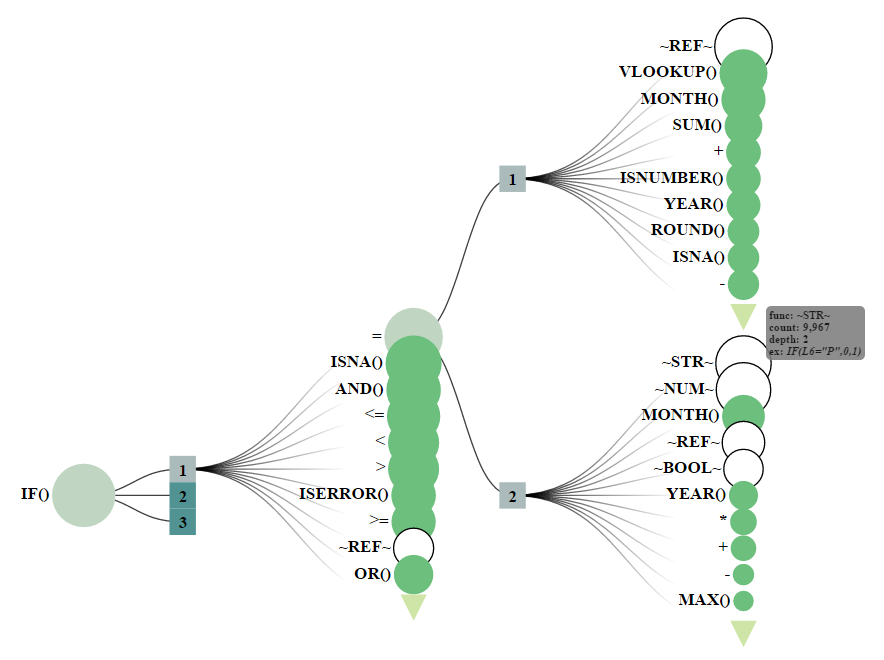
\includegraphics[width=0.8\textwidth]{IFargslabel}
		\caption{A picture of \toolname displaying the common arguments to the \texttt{IF}
			function's first parameter} \centering \label{fig:fullpic} \end{figure*}
	
	The equality operator has certain types of arguments
	which predominate over the others: on the left side is most often a reference
	to another cell; on the right is a string or number literal, which makes sense
	for the case of confirming a value in another cell before assigning this one.
	Furthermore, a tooltip accompanies each function node in the tree, providing a
	concrete example of a function that uses this structure. If this single
	instance is not enough, then the user also has the option to open up a new
	window with a table of many more examples from dataset.
	
	\subsection{Glyph Glossary}
	
	From these images, we provide glossary of glyphs to better interpret the visualizations. \begin{itemize} \item
		
\includegraphics{glossary-green} \textbf{Function nodes} are green circles
		labeled with the function name. Their size is determined by their relative
		frequency, scaled logarithmically, to the frequency of the root node in the
		tree. They may have any number of arguments, including zero, as determined by
		the API. Users can select any of these nodes to view the examples from the
		provided dataset that use this function in the node's position in the tree.
		
		\item \vspace{.25cm}
\includegraphics{glossary-leaf} \textbf{Value nodes} are
		white circles with a generic label. They represent elements of a formula that
		accept no arguments, like references (A1), ranges (A1:A10), numbers, boolean
		values, strings, and errors. However, \toolname still treats functions with
		zero arguments, like \texttt{NOW}, as function nodes. Like function nodes,
		these also link to examples.
		
		\item  \vspace{.25cm} 
\includegraphics{glossary-blue} \textbf{Argument nodes}
		are dark blue squares labeled with a number. The number is the position of an
		argument within the function of the parent node. In Figure~\ref{fig:expandif}
		for example, argument node 1 shows every function or value that was seen in
		the first argument.
		
		\item  \vspace{.25cm} 
\includegraphics{glossary-solidline} \textbf{Solid
			lines} represent a function's list of parameters. As such, they connect the
		function nodes to argument nodes.
		
		\item  \vspace{.25cm} 
\includegraphics{glossary-fadingline} \textbf{Fading
			lines} represents how a formula author can choose from several possible
		functions or values within a single argument position. As such, these lines
		connect argument nodes to function or value nodes.
		
		\item  \vspace{.25cm} 
\includegraphics{glossary-arrow} \textbf{Expansion
			arrows} appear within an argument node when there are over 10 possible
		functions or values in an argument position. By default, only the first 10
		will be shown along with this arrow; clicking this will show the rest as well.
		
		\item  \vspace{.25cm}
		$\vcenter{\hbox{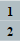
\includegraphics[scale=.75]{glossary-lightblue}}}$
		\textbf{Optional argument trees} are variations of trees that show only
		formulae with a specific number of arguments. For example, the function
		\texttt{AND} can take any number of arguments, up to 255. By default, the tree
		shows data from \texttt{AND} functions with any number of arguments, and an
		example of the \texttt{AND} tree with sample contents is shown on the left of
		Figure~\ref{fig:optional}. Optional argument trees, however, have argument
		nodes of a lighter blue color and show how \texttt{AND} was used when
		\textit{exactly} two arguments were passed into it, or \textit{exactly} four,
		without including uses of this function with any other number of arguments.
	\end{itemize}
	
	\begin{figure}[h] 
		\centering
		\begin{subfigure}
		  \centering
		  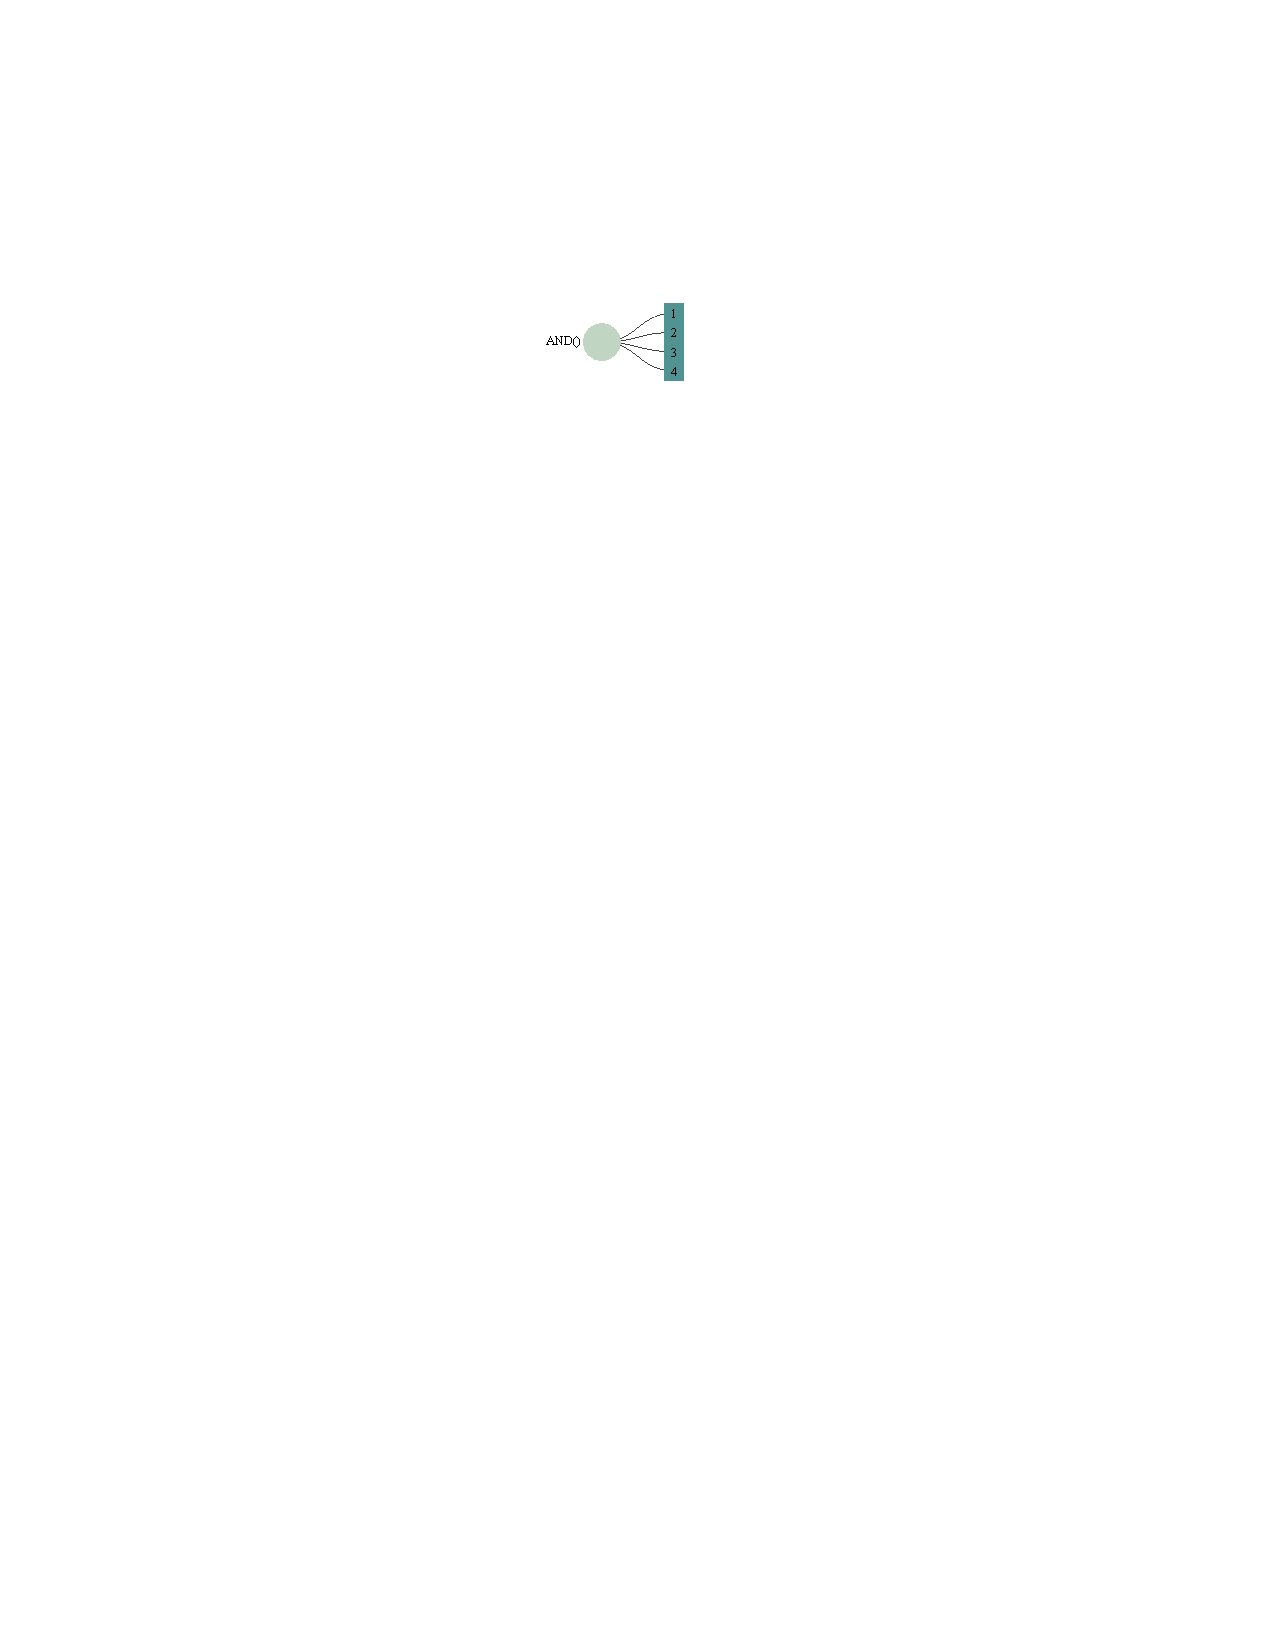
\includegraphics[width=.4\linewidth]{comparison1}
		\end{subfigure}%
		\begin{subfigure}
		  \centering
		  
\includegraphics[width=.4\linewidth]{comparison2}
		\end{subfigure} 
		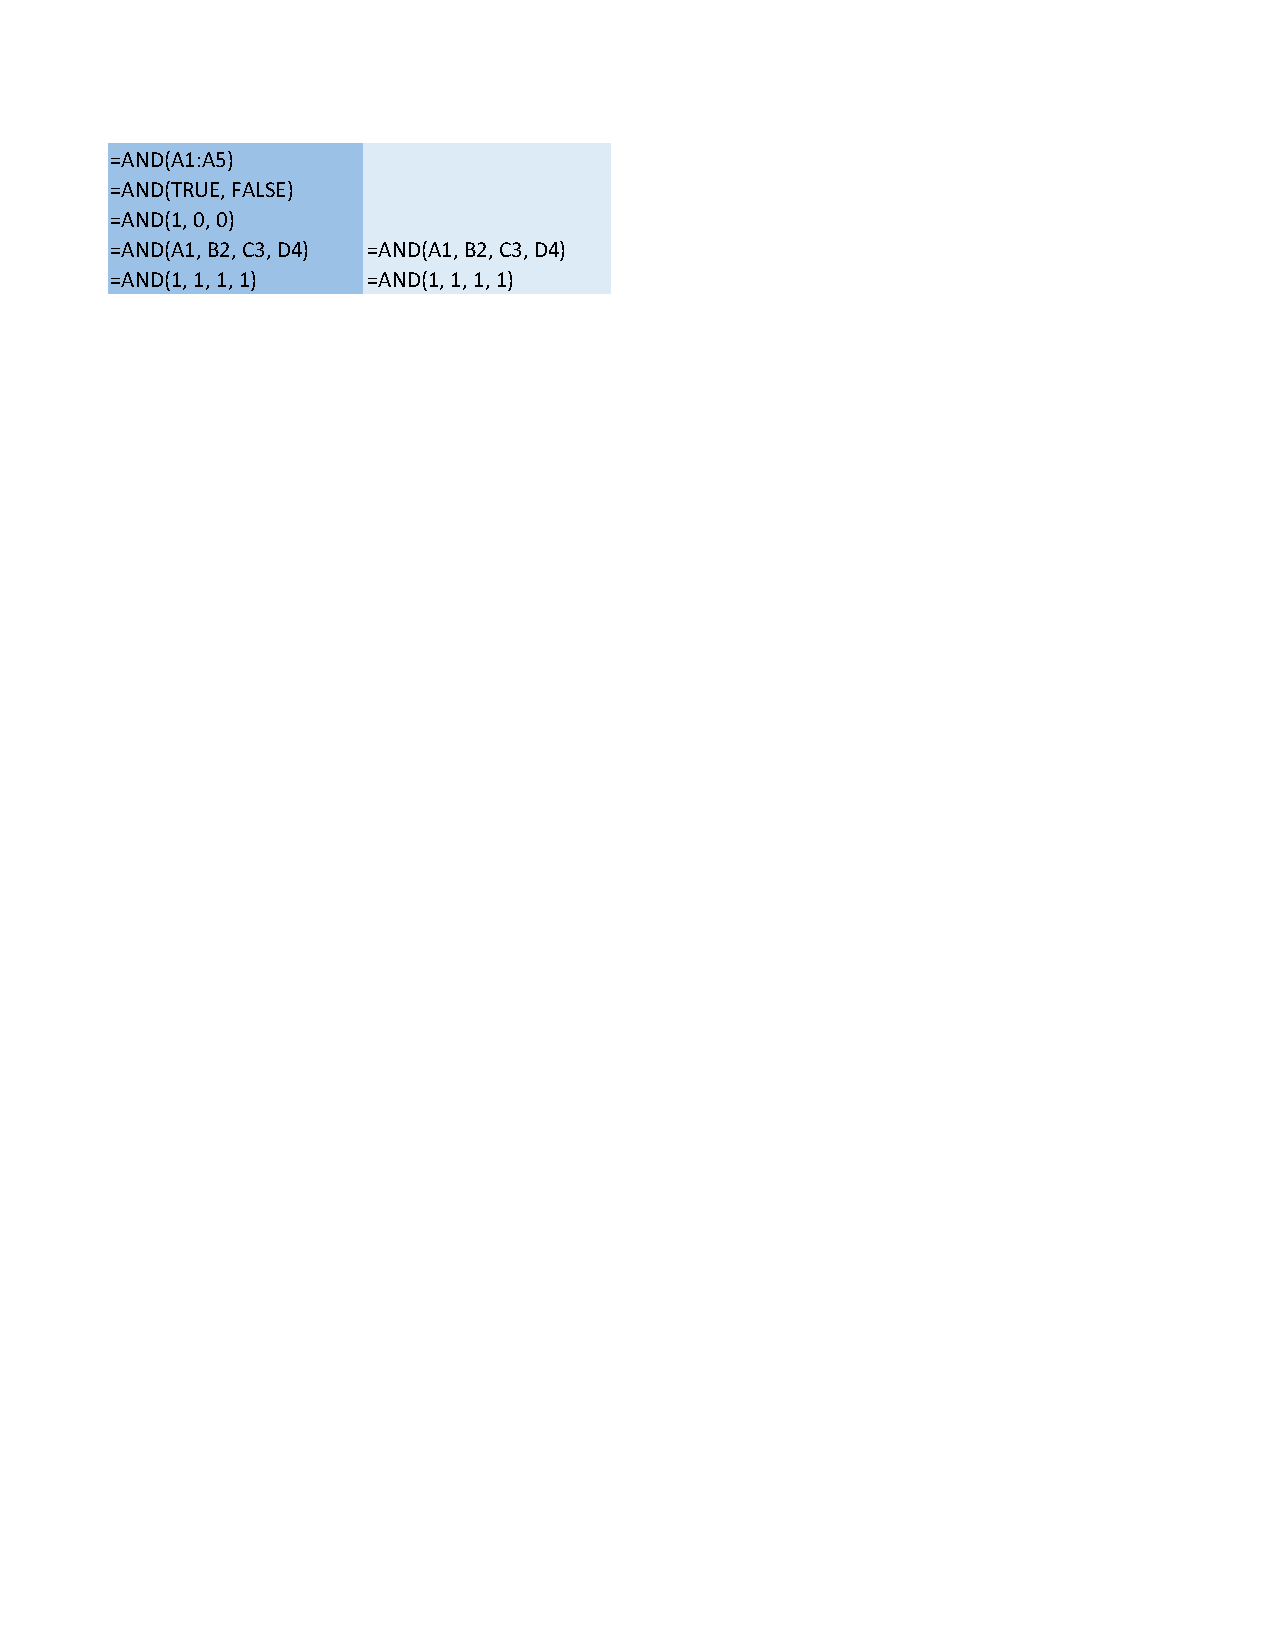
\includegraphics[]{comparison-ss} \caption{The
			contents of the default tree (left) and the optional argument tree with 4 arguments (right)}
		\label{fig:optional} \end{figure}
	
	
	
	\subsection{Implementation Details} The visualization is the product of two processes: \begin{itemize} \item \textit{Collection}: Given a set of
		Excel sheets, the tool, written in Java, uses Apache
		POI\footnote{\href{https://poi.apache.org/}{https://poi.apache.org/}} to identify and iterate over every cell
		containing a valid formula. Afterward, it calls POI's formula parser to decompose
		the formula text into an ordered set of individual tokens, which the tool then
		parses into the tree-like form. When all formulae have been analyzed like this,
		it produces JSON files for each top-level function in the set.
		
		\item \textit{Presentation}: The JSON files, meanwhile, feed into the
		presentation code, implemented in Javascript with much help from the
		visualization library D3\footnote{\href{https://d3js.org/}{https://d3js.org/}}. We chose D3 primarily
		for its accessibility: given the JSON, the visualization can be simply
		embedded into a webpage accessible through a browser. \end{itemize} A
	demonstration of \toolname can be found at
	\href{https://github.com/DeveloperLiberationFront/Excel-Function-Visualizer}{https://github.com/DeveloperLiberationFront/Excel-Function-Visualizer}.
	
	\subsection{Design Decisions} \label{ssec:decisions} Early in the design, we
	chose the tree form for its inherent ability to represent the parent-children
	relationship of formulae as functions and their arguments, which could be yet
	more functions. One option that we did not take was to represent the call trees
	as simple text hierarchies. Though that might work well for a single,
	uncomplicated call structure, we did not do this because our tool combined many
	of these call trees into a more complicated structure. To capture the different
	relationships in the tree and to quantify the frequency of arguments, we would
	need to be more verbose in our description. As such, we decided that
	visualizing some dimensions was quicker than writing them out.
	
	In balancing this chosen form with the goals in Section~\ref{goals}, we faced a
	number of decisions in how to visualize the data. Below, we've outlined those
	that had the largest impact in the values that appear in the tree.
	\begin{itemize}
		
		\item \textit{Copied formulae}: Excel allows users to spread a formula over an
		area, repeating the same formula in each cell with minor adjustments. Without
		checking for this, the analysis may not reveal the functions most commonly
		used together but rather the formulae most often applied to large areas. To
		combat this, we converted formulae from their native A1 format to the relative
		R1C1, in which copied formulae should be identical, and considered only each
		R1C1 formulae once per worksheet.
		
		\item \textit{Importance of depth}: When a function appears within another,
		should it be analyzed only as a nested function or should \toolname
		analyze the nested function as a top-level function as well? 
		
		\ \ For example, in the pictured \texttt{IF} function, we found that people often use
		another IF statement as the second or third arguments of the top-level \texttt{IF}. If
		we only consider functions exactly where they're found embedded in the
		formula, then information about the same function -- \texttt{IF}, in this case -- will
		be scattered across different trees with no way to aggregate them. If we
		record every instance of a function by ignoring their context -- that is,
		including an \texttt{IF} embedded within a \texttt{SUM} function in the same node as the
		top-level \texttt{IF} -- then the tool will represent some functions in multiple nodes
		to capture every possible level of nesting. For now, we only include the
		first, with the latter to be added as an option in the future.
		
	\end{itemize}
	
	\section{Case Study} The obvious question to pose any visualization is this:
	What do the images tell us that the text could not? It is not enough to prove
	that something can be visualized; we must also demonstrate what we can gain
	from any particular visualization. For this purpose, we outlined a few tasks in the
	introduction in which we thought the tool could help, particularly detecting bad smells and
	guiding spreadsheet education. To demonstrate the tool's applicability, we
	sought out places in the tree which best exemplify these tasks.
	
	\subsection{Bad Smells} \label{badsmells} Fowler's description of code
	smells~\cite{fowler2009refactoring} underscores an important point of code
	quality: between elegant, efficient code and bug-crippled spaghetti, there is a
	spectrum of code designs which, by themselves, are not faulty but nevertheless
	suggest problems in code design. Since then, researchers have applied
	these concepts to spreadsheet programming, as discussed in
	Section~\ref{related-work}. While some of the documented code smells lie beyond the scope of
	the tool, such as those characterizing inter-worksheet connections, others have
	structures which create distinctive features within the tree, leading to easy
	detection through our visualization: 
	
	\begin{itemize}
		
		\item \textit{Multiple Operations}: A single formula comprises numerous
		functions and operators~\cite{hermans2012detecting}. As a result, the formula
		tends to be complex. In the visualization, since each nested and
		combined function creates yet another level of depth within the tree, these
		constructions can result in long, horizontal chains of nodes, as seen in
		Figure~\ref{fig:longsum}.
		
		\item \textit{Long Parameter List}: A function uses numerous arguments, making
		it harder to understand~\cite{asavametha2012detecting}. This is not a problem
		for many functions which have a limited number of arguments that it accepts.
		However, for functions that accept arguments indefinitely, such as \texttt{SUM} and
		\texttt{CONCATENATE}, it creates tall towers of argument nodes from a single function
		node.
		
		\item \textit{Conditional Complexity}: A logical function, particularly \texttt{IF},
		nests several other logical functions inside of it, reducing code
		readability~\cite{hermans2012detecting}. These can be traced manually in the
		trees for the logical functions. \texttt{IF}, for example, will have several more \texttt{IF}
		function nodes within its second or third arguments, which in turn might have
		more of the same nested within them.
		
	\end{itemize}
	
	\begin{figure*}[h] \centering 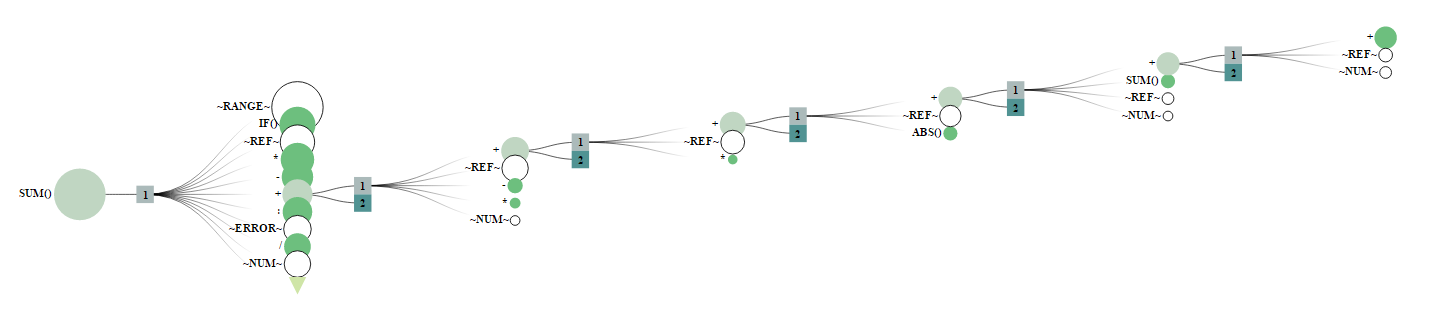
\includegraphics[width=\textwidth]{longsum}
		\caption{The horizontal length of a tree may indicate complex or redundant
			design} \label{fig:longsum} \end{figure*}
	
	Aside from these three, some code issues are meaningful not for the space they
	occupy but for how they clash with a function's expectations. For example,
	Excel offers a number of functions that accept as many arguments given to
	them, up to a resource-defined limit. \texttt{SUM}, for example, simply sums up every
	argument given to it. This also means that it can accept only one argument, and
	when the user does so, they pass in a range of cells over 90\% of the time.
	However, using \toolname, we found an instance where the programmer used a
	single-argument \texttt{SUM} where the argument was a series of 32 contiguous cells
	added with the + operation -- ``\texttt{SUM(C6+C7+C8+C9+C10+C11+C12+C13+...+C37)}" --
	representing a correct but redundant design.
	
	However, because \toolname makes no judgments beforehand about which designs to
	emphasize as good or bad, the tool can be used to find strange or suboptimal
	designs that exist outside these readily visible categories. Consider the
	second argument of the \texttt{``=''} operator, already shown expanded in
	Figure~\ref{fig:fullpic}: among the top five argument types for the position in
	an \texttt{IF} function were boolean values. This corresponds to designs in which
	conditions already in a boolean form were then checked against \texttt{``=TRUE"} or
	\texttt{``=FALSE"}, such as in the formula \texttt{IF(Formulas!C77=TRUE, ``Yes")}, which
	appears in one of the sheets. Though this practice does not break anything in
	itself, it nevertheless represents redundant operations in formula design and
	indicates a possible misunderstanding of how the IF function works.
	
	\subsection{Education} When Robillard and Deline researched common obstacles
	for programmers learning new APIs, they concluded that one of the most
	important elements of a good API was the use of code examples~\cite{robillard2011field}. Examples in APIs, furthermore, come in
	a variety of forms: small snippets or tutorials that show only the intended
	function, sample applications that incorporate the function in a broader
	context, or even production code that employs the function but was not
	initially intended to be an illustrative example. Of these categories,
	\toolname aligns entirely with the last; when a user chooses to explore a
	particular function node, they will see examples of that formula as it was used
	in a working environment, with the specifics depending on the dataset the tool
	is using. 

	Furthermore, Robillard and Deline's study makes the case for examples that show
	``API usage patterns involving more than one method
	call"~\cite{robillard2011field}. Examples that show only a single function,
	they find, are too simple, whereas those demonstrating the interaction of
	functions will equip users for more complex tasks. \toolname is especially
	suited for this focus on combination; consider again the question in the
	walkthrough (Section \ref{sec:walkthrough}), asking which functions and
	operations are used as conditions in IF. The design of this tool emphasizes the
	connection, then, between what functions like \texttt{ISNA} and \texttt{AND}
	return and what \texttt{IF} accepts, and specific examples for any of these
	combinations are only a click away.
	
	%Lookup example
	For a deeper example, the LOOKUP functions are some of the most popular in
	Excel yet come with a number of important but silent requirements for proper
	use, and, as such, they have warranted some extra attention with regards to
	spreadsheet design. In short, these functions are for ``when you need to look
	in a single row or column and find a value from the same position in a second
	row or
	column"\footnote{\href{https://support.office.com/en-us/article/LOOKUP-function-446d94af-663b-451d-8251-369d5e3864cb}{https://support.office.com/en-us/article/LOOKUP-function-446d94af-663b-451d-8251-369d5e3864cb}}. Examples of their use can be found in Figure~\ref{fig:lookupexample}, and we will cover each type in more depth to better understand the visualizations for these functions.
	
	\begin{figure}[h] \centering
		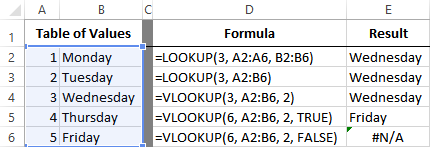
\includegraphics[width=.5\textwidth]{lookupexample} \caption{Demonstrations of
			LOOKUP and VLOOKUP} \label{fig:lookupexample} \end{figure}
	
	\texttt{LOOKUP} has two forms: vector and array. In either case, the first argument is
	the value which you are trying to match in another column. If the formula is in
	the vector form, that column is the second argument, so in
	Figure~\ref{fig:lookupexample}, the formula in cell D2 (\texttt{=LOOKUP(3,
		A2:A6, B2:B6)}) will search for the value of 3 between cells A2 and A6. The
	value that the formula returns then comes from the corresponding cell in the
	optional third argument's column; since the lookup values matches the value in
	cell A4, it returns the value from cell B4. The array form of the LOOKUP works
	the same way, except that the second argument is a two-dimensional table where
	it matches values in the table's first column and returns values from the last.
	Also, depending on the dimensions of the lookup table, the function may
	substitute rows for columns.
	
	\texttt{VLOOKUP} works closely with this array form, except the user defines in its
	third argument which column from which to return values. In \texttt{=VLOOKUP(3,
		A2:B6, 2)}, the argument ``2" tells to return the value from the second column,
	which is \textit{B2:B6} here. Furthermore, it also accepts a boolean value for
	an optional argument: when set to FALSE, it returns only exact matches, and
	when TRUE or left out, it approximates the match to the closest value beneath
	it. We demonstrate this in Figure~\ref{fig:lookupexample} in the bottom two
	\texttt{VLOOKUP} functions, one returning ``Friday" and the other an error. \texttt{HLOOKUP}
	works identically but focuses on rows instead of columns.
	
	All of these variations may seem daunting to a beginner, but \toolname can
	help. Because of its design, users can distinguish between forms of the same
	function, as seen in Figure~\ref{fig:lookups} where one can explore both the
	frequency with which the spreadsheet programmers used these different forms --
	three-argument vector form much more than the array form -- and then retrieve
	examples of every configuration in the dataset. The same goes for the \texttt{V/HLOOKUP}
	functions, as shown partially in Figure~\ref{fig:vhlookups}.
	
	\begin{figure}[h] \centering 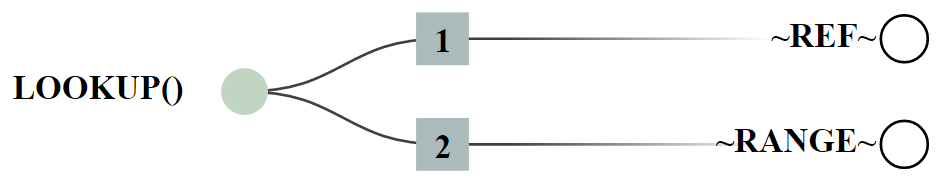
\includegraphics[width=.5\textwidth]{lookup-2}
		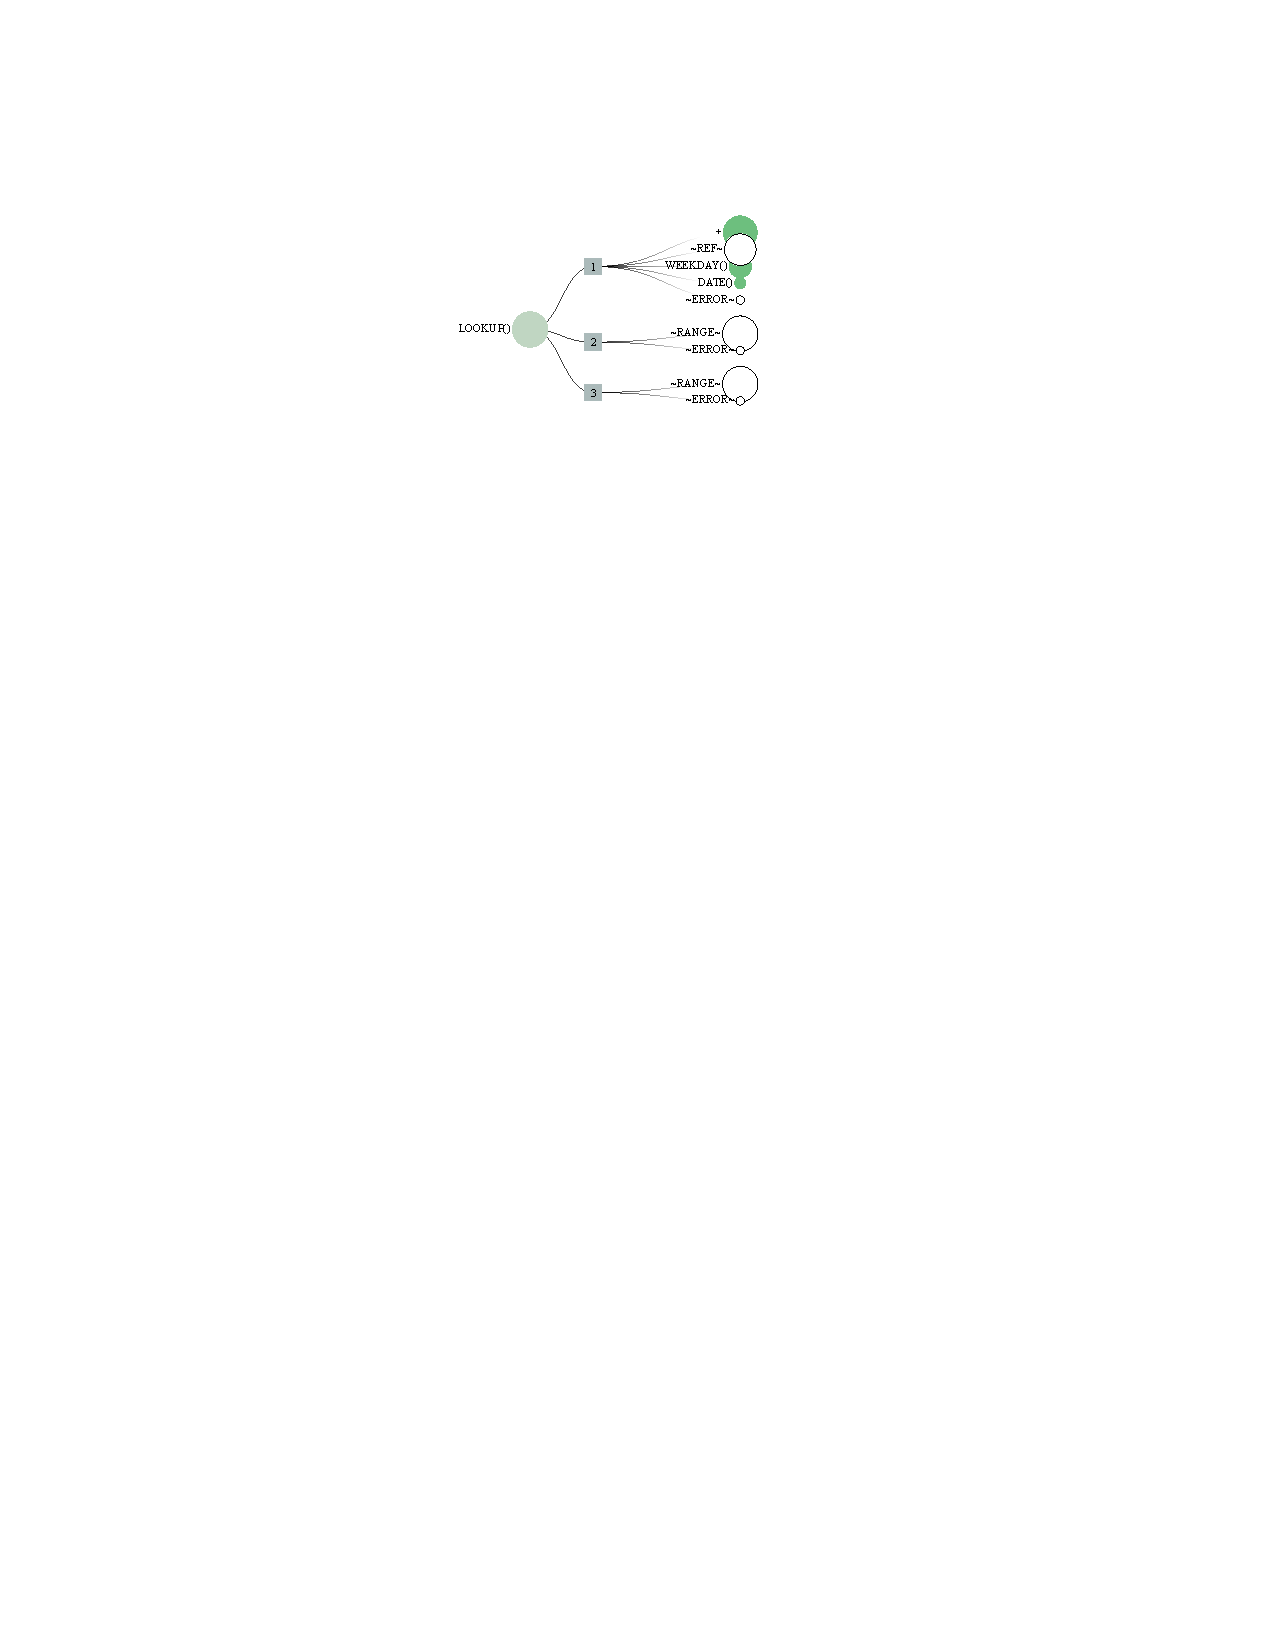
\includegraphics[width=.5\textwidth]{lookup-3} \caption{LOOKUP with two and
			three arguments}  \label{fig:lookups} \end{figure}
	
	Furthermore, these examples are good as well for exploring how it might bridge
	issues of bad design with education. In a recent study, Hermans and colleagues
	probed the Enron dataset for uses of VLOOKUP and HLOOKUP
	specifically~\cite{hermans2015detecting}. The issue at hand was the optional
	fourth argument, which requires that rows are sorted lest it return inaccurate
	results. For someone seeking to increase awareness of this problem, it first
	allows them to answer the question of significance -- ``How often do
	spreadsheet programmers use this function, with these particular parameters?"
	Though \toolname does not discern whether neighboring columns are sorted, it
	can nevertheless guide the educator to several examples in production where
	this problem surfaces. 
	
	\begin{figure}[h] \centering 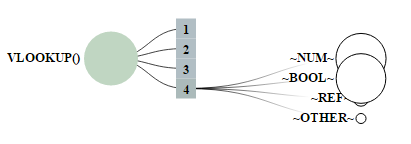
\includegraphics[width=.5\textwidth]{vlookup}
		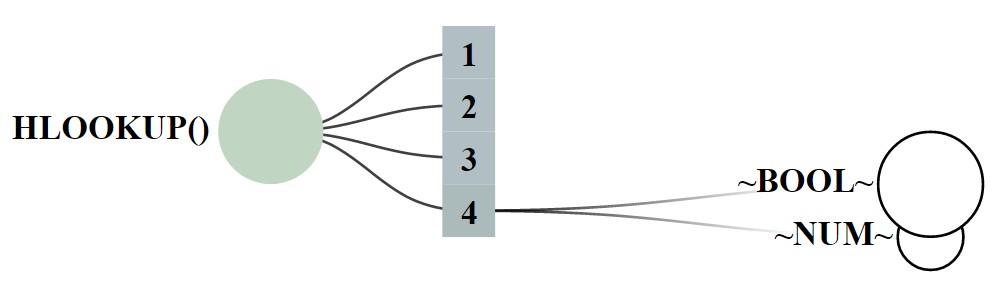
\includegraphics[width=.5\textwidth]{hlookup} \caption{VLOOKUP and HLOOKUP with
			four arguments} \label{fig:vhlookups}\end{figure}
	
	\section{User Study} \label{sec:userstudy} 

	We conducted a brief, exploratory user study during development to detect
	conflicts between our design and the goals in Section~\ref{goals}. In it, we
	gave the participants a set of visualizations from the Enron dataset and at
	least 20 minutes, and we asked them to adopt the persona of a consultant
	evaluating a company's spreadsheet practice. Through this framing, we intended
	to open the floor for questions like on which functions employees most depended
	and which sheets contained the most dangerous formula practice. We clarified,
	furthermore, that their observations could be directed either at the quality of
	the data conveyed by the tool or at the tool's design itself.
	
	We had four participants, labeled P1 through P4. Only P4 had no experience with
	spreadsheets in a professional environment, having used spreadsheets
	intermittently through education and hobbies. P1 through P3 all had varying
	levels of experience with spreadsheets in a professional capacity: P1 for 1
	year, P3 for 3, and P2 for 5. All participants were graduate students at the
	time of study but with some prior experience in industry, and we presented each
	with the same broad question about spreadsheet practice. Though interpretation
	of the phrase ``spreadsheet practice" can certainly vary from participant to
	participant, we readily accepted this interpretive flexibility since we wanted
	a range of views and backgrounds despite the persona. Furthermore, their
	differing levels of expertise let us judge the accessibility of the
	visualization; even if a participant had no formal knowledge of code smells, we
	found it valuable nevertheless if they could intuitively identify bad design.
	
	\subsection{Use in Smell Tracking}
	
		\begin{wrapfigure}{O}{.25\textwidth} \centering
			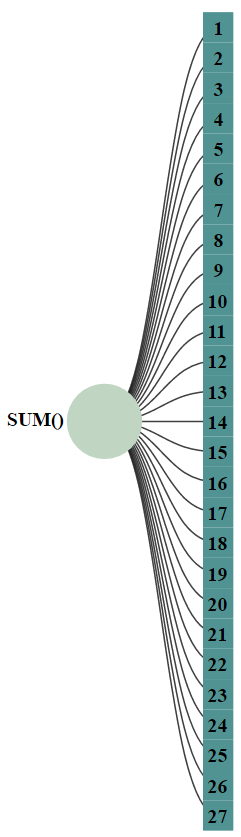
\includegraphics[width=.20\textwidth]{SUM}  \caption{An abundance of parameters
				in SUM, which was a commonly noted smell in the user study} \label{fig:sum}
		\end{wrapfigure}

	The participants were most vocal about their findings when they discovered
	instances of design they considered problematic. Many times, they noted these
	examples shortly after opening a new tree, suggesting that the distinctive
	visual signatures of code smells as discussed in Section~\ref{badsmells} were a salient force
	in their exploration. For example, when P3 encountered the
	initial design of the SUM tree, as seen in Figure \ref{fig:sum}, they readily
	diagnosed that either a spreadsheet author was ``totally incompetent, or [the
	formula was] just something that's weird." Even though the visualization
	struggles to scale well for this formula, it calls clearly to a problem in the
	underlying spreadsheets -- awkward formulae make awkward trees. Other than
	these visual cues, value errors, prefixed with \#s, also appear in the tree,
	which P4 said could be useful for tracking these problems if they're easy to find.
	
	Additionally, because the Enron files had names with the author as a prefix, P2
	commented that companies could use the tool to follow up with repeat offenders.
	For instance, they first encountered a particular author's name when
	investigating an \texttt{AVERAGE} function with 18 distinct arguments for which our
	participant could not discern any logical order even after opening the source
	spreadsheet; the same name popped up again as P2 looked at a \texttt{RATE} function
	relying on several hard-coded values. P2 said that, if they were a manager or
	project leader, this recurrence was a sign to talk to the author personally and
	figure out why these problems were there, as to prevent more in the future.
	They also added that these problems would grow worse if this particular author
	left the company and no one remained who understood these formulae, a concern
	that aligns with Hermans' transfer scenarios \cite{hermans2011supporting}.
	
	The detection of bad design, however, is certainly not limited to a
	visualization tool. Some users remarked that a tool which printed a list of
	errors could work just as well for that purpose, and smell checkers can and
	have been directly built into spreadsheets to point out bad design. However,
	users also said that this visual interface is better when searching for new
	smells. Because the exploratory design makes no qualitative judgment and
	visualizes benign designs with the problematic, it allows for flexible
	interpretation of what a smell is; that is, a user might not realize a certain
	design is poor until they see it in the tree and, at the point, find specific
	examples of where it occurs in the spreadsheets.
	
	\subsection{Use in Education} Users found \toolname's inclusion of examples to
	be especially useful since none of the them considered themselves to be experts
	of Excel, their self-reported proficiencies ranging from ``fairly familiar"
	(P2) to ``not extremely familiar" (P4). For example, as P1 explored the \texttt{VLOOKUP}
	function, they said they could use the tool to collect more examples than the
	documentation offers even though they knew the documentation more verbosely
	explained its function signature. Furthermore, in the process of exploring
	trees, P1 and P3 also gravitated towards some functions they had not used
	before, such as \texttt{PV} and \texttt{IPMT}, looking for new features in Excel to explore and
	learn. 
	
	Additionally, \toolname offers a simple way of finding examples where certain
	functions were used together, demonstrated when P4 took special interest in how
	people frequently used \texttt{MATCH} as the second argument of \texttt{INDEX} or how they used
	date functions like \texttt{DATE} and \texttt{MONTH} as lookup values in \texttt{VLOOKUP}. Though a
	standard text-search tool might yield the same results for a function alone,
	combinations can require more complex text queries, whereas here, the
	information is already captured in nodes. 
	
	However, we found that even though a user can explore all of a function's
	configurations, this does not mean that they will learn exactly what it does.
	P1, examining unfamiliar functions like\texttt{KURT} and \texttt{PV}, could describe precisely
	what types of arguments it accepted and how many. But even after exploring the
	spreadsheets for context, they could not accurately describe what the functions
	produced without consulting the official documentation. Whether through
	reticence of the tool or obscurity of the functions themselves, the exploratory
	environment is not enough to teach users \textit{when} to use a function.
	However, we could address this in future designs, perhaps, by linking directly
	to such documentation from within the tool without violating any design
	concerns in Section~\ref{goals}. 
	
	\subsection{Study Limitations} \label{subsec:studylimitations} 
	
	In a few ways, these user studies might not fully assess \toolnameposs value.
	For example, though we did not preface the study by revealing the source of the
	files, two users studied the file names to deduce its roots in finance, if not
	Enron itself. Because of these notorious connotations, then, they might have
	been inclined to orient their exploration around financial functions,
	potentially restricting their findings. However, one of these participants also
	said that they could not have intelligently explored a dataset in the first
	place without this essential context. Comments like these point out the
	trade-offs of unguided exploration, too: though it might not restrict them to a
	single purpose, it might, at the same time, not afford them any mindset at all
	with which to interpret the data. 
	
	Throughout the study, we noticed that users misunderstood the design
	and, as such, their early discoveries were inaccurate. For example, P1
	thought that the numbers on argument nodes as the number of arguments instead
	of the index of that argument -- that is, clicking on the dark blue
	``1" would return all the single-argument functions instead of the function's
	first argument -- and P2 initially took the solid lines to mean
	different paths in formula construction rather than different arguments of the
	same function. Though these misunderstandings were useful in pinpointing weak
	parts of the tool, their presence affected many of the participant's observations before we
	could clarify, reducing the amount of useful information from these sessions.
	
	\section{Tool Limitations} 
	
	We began these studies with the intention of evaluating
	our progress towards the goals in Section~\ref{goals}. Working from these
	results, we noted many places where \toolname itself aligned well or fell short.
	
	\subsection{Unbiased Exploration} 
	
	The goal of \toolname is exploration without bias, gap, or interruption, but 
	this version does not solve everything. First, \toolname cannot reliably
	salvage every formula. When a formula arises that the POI parser cannot handle,
	whether because of typos or third-party functions, the entire formula is lost;
	\toolname gets either the full formula or nothing at all. Second, while we 
	hard-coded nothing that explicitly emphasizes bad design, the nature of the
	visualization draws attention towards certain offenses, like those in
	Section~\ref{badsmells}. While these may be fairly obvious, however, they 
	may distract from subtler, more insidious patterns.
	
	Despite this second point, our participants found the discovery of bad smell
	to be the most interesting aspect about it. To design in that
	direction, however, would mean a reevaluation of this design goal, since
	intentionally guiding users toward known smells may guide them away from new,
	unmarked ones.
	
	\subsection{Uncluttered Quantification}
	
	We wanted to show everything, but everything overwhelms. We realized that danger
	early on and included features, such as the expansion arrows and the use of generic types
	instead of values, that would manage the variation. Nevertheless, P2 and P3 remarked
	that they often avoided the most popular functions, anticipating a flood
	of nodes from which they could salvage nothing interesting. P2 corroborated
	this by explaining how they preferred to explore specific examples in
	individuals nodes instead of navigating the full, crowded tree. Despite our
	precautions, balancing the desire to show a lot with the desire not to
	overwhelm remains a challenge.
	
	Some visual cues turned out to be more confusing than helpful, such as
	the index number on each argument node. As discussed in Section~\ref{subsec:studylimitations},
	users often mistook it for other features, like total number of arguments in the
	function. Though we kept this feature present for all studies, future versions
	of \toolname would refine this design. 
	
	\subsection{Informative Qualification}
	
	As we found in the case study, the tool excels at making formula examples
	available throughout a tree. However, the benefits described in the previous
	sections imply a hidden complication: if the tool educates through example but
	does not explicitly distinguish between good design and bad design, how can we
	be sure that people will not inadvertently learn bad design from it? In the
	user study, we discussed \toolnameposs use in education and smell detection by bringing
	up the issues surrounding the LOOKUP functions. This discussion, though,
	assumes a distinguishing eye that knew which examples practiced good design
	and which exhibited the common errors. A beginner might not know the
	difference. Robillard and Deline, in their study, remarked that good API
	examples should demonstrate best practices, but, right now, we have no way to
	assure this with \toolnameend. As with the problems in achieving unbiased
	exploration, correcting for this danger may entail a reevaluation of design
	goals.
	
	\section{Future Work}
	
	For these user and case studies, we relied solely on one type of spreadsheet (Excel)
	from one source (Enron), but we have room to develop in either dimension. For sources, 
	Enron's focus on finances and energy represents one context in
	which people use spreadsheets, but other corpora, like EUSES and Fuse, draw from
	other domains and industries. As Jansen found in his comparison of
	spreadsheets Enron and EUSES \cite{jansen2015enron}, different companies rely
	on different functions. For other types of spreadsheet, such as Gnumeric\footnote{\href{http://www.gnumeric.org/}{http://www.gnumeric.org/}} or Google
	Sheets\footnote{\href{https://www.google.com/sheets/about/}{https://www.google.com/sheets/about/}}, we have no
	guarantee that practices and functions will hold across these varied programs, even within
	similar domains. This, then, warrants further analysis, in which good visualization might serve
	well. 
	
	\begin{figure} \centering 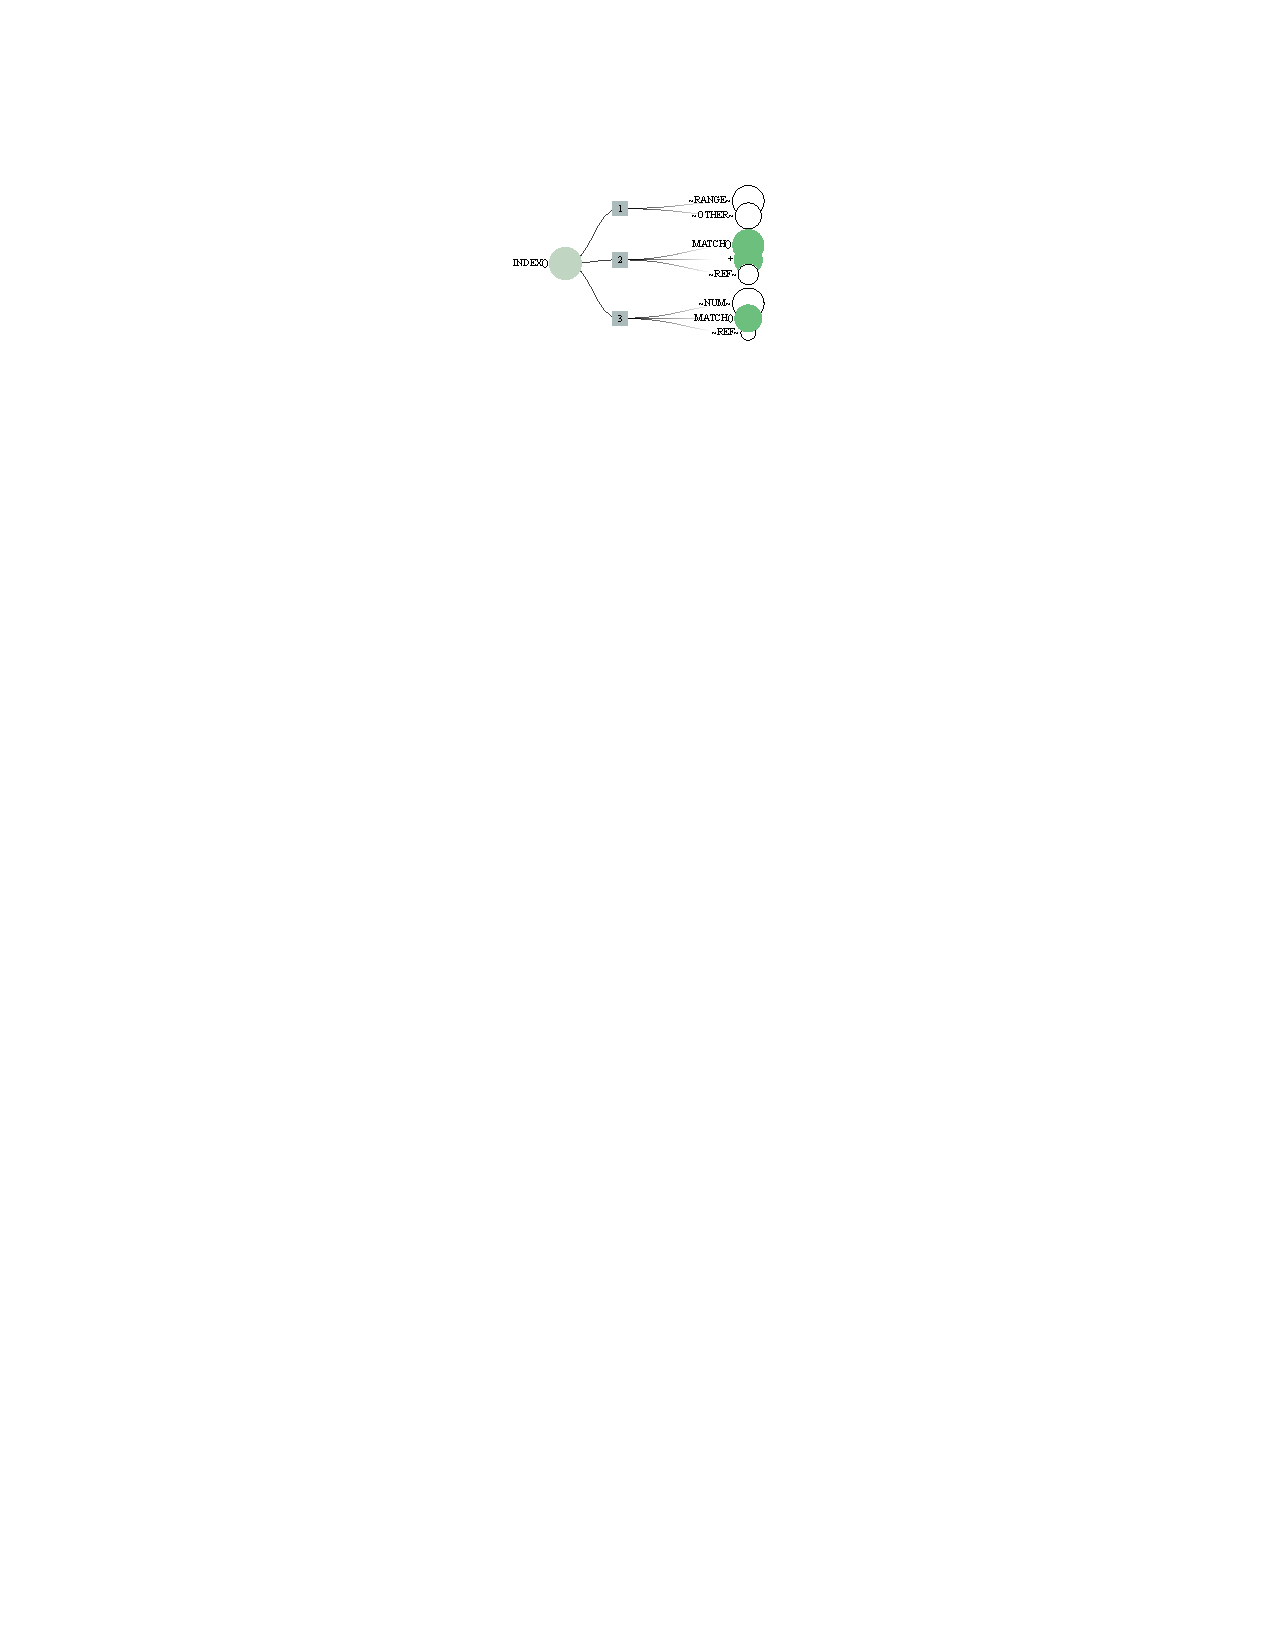
\includegraphics[width=.4\textwidth]{index}
		\caption{A difficult question: how often is MATCH used in both the second and
			third arguments?} \label{fig:index} \end{figure}
	
	Though our focus was specifically on function combination, there are several
	other elements of a formula's context that we do not currently consider. For
	example, \toolname does not current capture argument combination; in Figure
	\ref{fig:index}, it is impossible to state how often the function MATCH
	occurred in both the second and third arguments or whether they were more often
	paired with references. Furthermore, it is easy to open a tree and see what is
	used inside of a specific function, but finding information on what a function
	is used inside of takes considerably more work -- we see again in Figure
	\ref{fig:index} that MATCH is used inside INDEX, but we cannot know which
	functions have INDEX inside them without searching every other tree. More
	distant concerns might be exploring which functions often occur in adjacent
	cells in the sheet -- whenever INDEX occurs, which functions are seen most
	often in the cells around it?
	
	\section{Conclusion}
	
	This paper presents a tool to support the exploration of function combinations
	throughout a given spreadsheet dataset. By taking an agnostic approach to
	design quality, it attempts to convey the dataset's spreadsheet practices as
	is: the common along with the anomalous, and the well-designed along with the
	odorous. As seen in the user and case studies, this allows it to take on
	several potential roles at once, such as an environment for investigating code
	smells as well as a repository for examples for learning new techniques.
	
	The design of the tool still has much room for improvement. Though the
	exploratory philosophy fostered certain goals well, such as the ability to
	discover new problematic smells without knowing beforehand what they are, it
	hindered others. Some users, for example, found the trees of popular functions
	to be too crowded to explore well, or that their intention to use the tool to
	examine the good or the bad design exclusively was not fully supported by a
	tool that claimed to know neither. Many of the problems, however, were not
	essential to this design conflict and will be overcome in future iterations of
	design by refining icons and improving maneuverability.
	
	Either way, the visualization of these large datasets represents an important
	step in improving practice overall. By taking these voluminous oceans of data
	offered in spreadsheet corpora and rendering them comprehensible through
	visualization, we seek to draw attention to valuable information that would
	otherwise go unnoticed.
	
	% use section* for acknowledgment
	\section*{Acknowledgment}
	
	This material is based upon work supported in whole or in part with funding
	from the Laboratory for Analytic Sciences (LAS). Any opinions, findings,
	conclusions, or recommendations expressed in this material are those of the
	author(s) and do not necessarily reflect the views of the LAS and/or any agency
	or entity of the United States Government. We also thank the anonymous reviewers
	who advised the direction of this paper, the study participants for their comments,
	and Shivom Gargava for his help.
	
	% references section
	
	% can use a bibliography generated by BibTeX as a .bbl file
	% BibTeX documentation can be easily obtained at:
	% http://mirror.ctan.org/biblio/bibtex/contrib/doc/
	% The IEEEtran BibTeX style support page is at:
	% http://www.michaelshell.org/tex/ieeetran/bibtex/
	\bibliographystyle{IEEEtran} % argument is your BibTeX string definitions and
	% bibliography database(s)
	\bibliography{paper} %
	% <OR> manually copy in the resultant .bbl file
	% set second argument of \begin to the number of references
	% (used to reserve space for the reference number labels box)
	%\begin{thebibliography}{1}
	%
	%\bibitem{IEEEhowto:kopka}
	%H.~Kopka and P.~W. Daly, \emph{A Guide to \LaTeX}, 3rd~ed.\hskip 1em plus
	%  0.5em minus 0.4em\relax Harlow, England: Addison-Wesley, 1999.
	%
	%
	%\end{thebibliography}
	
	
	
	
	% that's all folks
\end{document}

